
\newpage
\section{Calculus}

\subsection{Differentation and Integration}
\bigskip


\begin{lemma}[Basic Formulas]\hfill
    \begin{enumerate}
        \item For \( 1 = x x^{-1} \) the product rule yields \( 0 = x^{-1} + x(x^{-1})' \). Hence
              \[
                  \frac{d}{dx} x^{-1} = -\frac{1}{x^2}
              \]
        \item Similarly \( x = \sqrt{x}^2 \) and \( 1 = 2 \sqrt{x} \sqrt{x}' \) and so
              \[
                  \frac{d}{dx} \sqrt{x} = \frac{1}{2\sqrt{x}}
              \]
        \item It is
              \[
                  \frac{d}{dx} x^n = nx^{n - 1}
              \]
              since via induction the product rule yields
              \[
                  \frac{d}{dx} x^n = \frac{d}{dx} xx^{n -1} = x^{n -1} + \frac{d}{dx} x^{n - 1} =
                  x^{n -1} + (n - 1)x^{n - 1}  = nx^{n - 1}
              \]
        \item Again, applying the product rule gives
              \[
                  \left(\frac{1}{g}\right)' = \left(\frac{1}{x} \circ g\right)' = -\frac{g'}{g^2}
              \]
              and the quotient rule
              \[
                  \left(\frac{f}{g}\right)' = \frac{f'}{g} + f \left(\frac{1}{g} \right)' =
                  \frac{f'}{g} -\frac{fg'}{g^2} = \frac{gf'- fg'}{g^2}
              \]
        \item Also \( x = f \circ f^{-1} \) and \( 1 = (f^{-1})'f' \circ f^{-1} \). Thus
              \[
                  (f^{-1})' = \frac{1}{f' \circ f^{-1}}
              \]
              where defined. Especially for \( x \ne 0 \)
              \[
                  \log'(x) = \frac{1}{\exp'(\log(x))} = \frac{1}{x}
              \]
        \item \( (1 - q) (1 + q + q^2 + \cdots + q^n) = 1 - q + q - q^2 + q^2 - q^3 + \cdots + q^{n+1} \) gives
              \[
                  \sum_{k=0}^n q^k = \frac{1 - q^{n+1}}{1 - q} \text{ and }
                  \sum_{k=m}^n q^k = \frac{q^m - q^{n+1}}{1 - q}
              \]
    \end{enumerate}
\end{lemma}
\bigskip


\begin{lemma}[Cauchy-Schwarz Inequality]\label{thm:lem_cauchy_schwarz_inequality}
    For \( x, y \in \Rn \) the following inequality holds
    \[
        |xy| \le \|x\| \|y\|
    \]
    Equality occurrs iff \( y \) is a multiple of \( x \).
\end{lemma}
\begin{proof}
    Assume \( xy = x_1 y_1 + \cdots + x_n y_n > 0 \). Then the inequality above is equivalent to
    \[ 0 \le 1 - \frac{xy}{\|x\| \|y\|} \]
    Here
    \[
        \begin{split}
            2 - \frac{2xy}{\|x\| \|y\|}
            & = \frac{x_1^2 + \dots x_n^2}{{\|x\|}^2} +
            \frac{y_1^2 + \dots y_n^2}{{\|y\|}^2} - \frac{2x_1 y_1 + \cdots + 2x_n y_n}{\|x\| \|y\|} \\
            & = {\left( \frac{x_1}{\|x\|} - \frac{y_1}{\|y\|} \right)}^2 + \cdots +
            {\left( \frac{x_n}{\|x\|} - \frac{y_n}{\|y\|} \right)}^2
        \end{split}
    \]
    Similarly for \( xy < 0 \). Note, that \( xy > 0 \) implies \( \lambda > 0 \) for \( x = \lambda y\).

    Of course, using \( xy = \|x\| \|y\| \cos\alpha \) is easier once this formula has been established.

\end{proof}
\bigskip


\begin{lemma}[Triangle Inequality]\label{lem:triangle_inequality}
    For \( x, y \in \Rn \) the following inequality holds
    \[
        \|x + y\| \le \|x\| + \|y\|
    \]
\end{lemma}
\begin{proof}
    It is
    \[
        {\|x + y\|}^2 = {\|x\|}^2 + 2xy + {\|y\|}^2 \le {\|x\|}^2 + 2|xy| + {\|y\|}^2
        \le {\|x\|}^2 + 2\|x\| \|y\| + {\|y\|}^2 = {(\|x\| + \|y\|)}^2
    \]
\end{proof}
\bigskip


\begin{remarks}Let \( f \) be differentiable at \( x_0 \). From the definition follows
    \begin{enumerate}
        \item \( f \) is \emph{Lipschitz continous} at \( x_0 \), e.g.\ there exists a \( L > 0 \) so that
              \( |f(x) - f(x_0)| < L|x - x_0| \) in some small enough environment of \( x_0 \).
        \item If there exists a sequence  \( x_n \to x_0 \) with \( f(x_n) = f(x_0) \) then \( f'(x) = 0 \).
              Consequently, if \( f'(x) \ne 0 \) then \( f(x) \ne f(x_0) \) in some local environment of \( x_0 \).
    \end{enumerate}
\end{remarks}
\bigskip

\begin{lemma}[Chain Rule]
    The chain rule for differentiable functions \( f \) and \( g \) yields
    \[
        (f \circ g)'(x) = f'(g(x))\, g'(x)
    \]

    \begin{proof}
        For \( g'(x_0) \ne 0 \) there exists a local environment of \( x_0 \) where
        \[
            \frac{f(g(x)) - f(g(x_0))}{x - x_0} =
            \frac{f(g(x)) - f(g(x_0))}{g(x) - g(x_0)} \frac{g(x) - g(x_0)}{x - x_0}
        \]
        Otherwise the remark above gives
        \[
            \left| \frac{f(g(x)) - f(g(x_0))}{x - x_0} \right| \le
            L\left| \frac{g(x) - g(x_0)}{x - x_0}  \right|
        \]
        and \( (f \circ g)'(x_0) = 0 \).
    \end{proof}
\end{lemma}
\bigskip


\begin{lemma}[Exponential Function]\hfill
    \begin{enumerate}
        \item It is
              \[
                  \exp(x + y) = \exp(x)\exp(y)
              \]
              Hence
              \[
                  \exp(0) = 1
              \]
              \[
                  \exp(-x) = {\exp(x)}^{-1}
              \]
              \[
                  \exp(nx) = {\exp(x)}^n
              \]
        \item For the derivative
              \[
                  \exp'(x) = \sum_{k=0}^\infty \frac{1}{k!} (x^k)' = \sum_{k=0}^\infty \frac{1}{k!} kx^{k-1}
                  = \sum_{k=1}^\infty \frac{1}{(k-1)!} x^{k-1} = \exp(x)
              \]
    \end{enumerate}
\end{lemma}
\bigskip


\begin{lemma}[Sinus and Cosinus]\hfill
    \begin{enumerate}
        \item Sinus and Cosinus power series
              \[
                  \begin{split}
                      \cos(x) &= \sum_{k=0}^\infty \frac{{(-1)}^k}{2k!} x^{2k} \\
                      \sin(x) &= \sum_{k=0}^\infty \frac{{(-1)}^k}{(2k + 1)!} x^{2k + 1}
                  \end{split}
              \]
        \item Symmetry
              \[
                  \begin{split}
                      \cos(-x) &= \sum_{k=0}^\infty \frac{{(-1)}^k}{2k!} {(-x)}^{2k} = \cos(x) \\
                      \sin(x) &= \sum_{k=0}^\infty \frac{{(-1)}^k}{(2k + 1)!} {(-x)}^{2k + 1} = -\sin(x)
                  \end{split}
              \]
        \item Derivatives
              \[
                  \begin{split}
                      \cos'(x) &= \sum_{k=1}^\infty \frac{{(-1)}^k}{(2k - 1)!} x^{2k - 1}
                      = \sum_{k=0}^\infty \frac{{(-1)}^{k + 1}}{(2k + 1)!} x^{2k + 1} = -\sin(x) \\
                      \sin'(x) &= \sum_{k=0}^\infty \frac{{(-1)}^k}{2k!} {x}^{2k} = \cos(x)
                  \end{split}
              \]
    \end{enumerate}
\end{lemma}
\bigskip


\begin{theorem}[Fermat Stationary Point]\label{thm:fermat_stationary_point}
    Let \( \Omega \subseteq \R \) be open and \( f \in C^1(\Omega) \). If \( x^* \in \Omega \) is local extremum
    then \( f'(x^*) = 0 \).
\end{theorem}

\begin{proof}
    Assume \( x^* \) is the minimum of \( f \) in \( \Omega \) and let \( f(x^*) > 0 \).
    Since \( f \in C^1(\Omega) \) there exist \( \eps, \delta > 0 \) so that for \( |h| \le \eps \)
    \[
        \frac{f(x^* + h) - f(x^*)}{h} > \delta
    \]
    Pick a negative \( h \in [-\eps, 0) \). Then   % chktex 9 
    \[
        f(x^* + h) < f(x^*) +  \delta h < f(x^*)
    \]
    and \( x^* \) cannot be the minimum. Analog for maximum with a positive \( h \), then apply to \( -f \).
\end{proof}
\bigskip


\begin{theorem}[Rolle]\label{thm:rolle}
    Let \( f \in C[a,b] \) with \( f(a) = f(b) \). If \( f \) is differentiable in \( (a, b) \) then
    there exists a \( \xi \in (a,b) \) with \( f'(\xi) = 0 \).
\end{theorem}

\begin{proof}
    Assume \( f \) is not constant. Since \( [a,b] \) is compact there exists either a global minimum or maximum
    \( \xi \in (a,b) \) and Theorem~\ref{thm:fermat_stationary_point} can be applied.
\end{proof}
\bigskip


\begin{theorem}[Mean Value]\label{thm:mean_value}
    Let \( f \in C[a,b] \) be differentiable in \( (a, b) \). Then there exists a \( \xi \in (a,b) \) with
    \[
        f'(\xi) = \frac{f(b) - f(a)}{b - a}
    \]
\end{theorem}

\begin{proof}
    Apply Theorem~\ref{thm:rolle} to
    \[
        g(x) = f(x) - \frac{f(b) - f(a)}{b - a} (x -a)
    \]
\end{proof}
\bigskip


\begin{remarks}\hfill
    \begin{enumerate}
        \item More generally choose any \( \varphi \in C^1[a,b] \) with \( \varphi(a) = 0 \) and
              \( \varphi(b) = f(b) - f(a) \). Set \( g(x) = f(x) - \varphi(x) \) to see there is a \( \xi \in (a,b) \)
              with \( f'(\xi) = \varphi'(\xi)\).
        \item Let \( f \) be differentiable in \( (a, b) \) with \( f' = 0 \). For any \( x, y \in (a, b) \)
              \[
                  0 = f'(\xi) = \frac{f(y) - f(x)}{y - x}
              \]
              and \( f \) is a constant.
        \item Another useful generalization: let \( \Omega \subseteq \Rn \) be open and \( f \in C^1(\Omega) \). For
              \( x, y \in \Omega \) define \( \varphi(t) = f(tx + (1 - t)y) \) and apply the chain rule for differentiation
              \[
                  \varphi'(\xi) = \gradient {f(\xi x + (1 - \xi)y)}^T(x - y) = f(x) - f(y)
              \]
        \item The Cauchy Schwarz inequality then yields
              \[
                  \|f(x) - f(y)\| \le \|\gradient f(\xi x + (1 - \xi)y)\| \|(x - y)\|
              \]
    \end{enumerate}
\end{remarks}
\bigskip


\begin{theorem}[Differentiation Theorem]\label{thm:differentiation}
    Let \( f \in C[a,b] \) and define
    \[
        F(x) = \int_a^x f(t)\,dt
    \]
    Then \( F \in C^1[a,b] \) with \( F'(x) = f(x) \) for \( x \in [a,b] \).
\end{theorem}

\begin{proof}
    Applying the Mean Value Theorem of Integration gives
    \[
        F(x + h) - F(x) =  \int_x^{x + h} f(t)\,dt = f(\xi) h
    \]
    for some \( \xi \in (x, x + h) \).
\end{proof}
\bigskip

\begin{theorem}[Fundamental Theorem of Calculus]\label{thm:fund_calculus}
    Let \( F \in C^1[a,b] \) with \( F' = f \)  Then
    \[
        F(b) -F(a) = \int_a^b f(t)\,dt
    \]
\end{theorem}
\bigskip


\begin{lemma}
    For \( F' = f \) the product and chain rule for differentiation yield
    \begin{enumerate}
        \item Integration by parts
              \[
                  \int fg = Fg - \int Fg'
              \]
        \item Integration by substitution
              \[
                  F \circ \varphi = \int f\circ \varphi \cdot\varphi'
              \]
    \end{enumerate}
\end{lemma}
\begin{proof}
    It is \( (Fg)' = F'g + Fg' = fg + Fg' \) and
    \( (F\circ \varphi)' = F'\circ \varphi \cdot\varphi = f\circ \varphi \cdot\varphi \).
\end{proof}
\bigskip


\begin{examples}\hfill
    \begin{enumerate}
        \item Let \( f = g = \sin(nx) \). Then \( F = -1/n \cos(nx) \) and
              \[
                  \begin{split}
                      \int \sin^2(nx)\,dx
                      & = -\frac{1}{n} \cos(nx)\sin(nx)\dx + \int \frac{1}{n} \cos(nx) n \cos(nx)\dx \\
                      & = -\frac{1}{n} \cos(nx)\sin(nx)\dx + \int \cos^2(nx)\dx \\
                      & = -\frac{1}{n} \cos(nx)\sin(nx)\dx + \int 1 - \sin^2(nx)\dx
                  \end{split}
              \]
              Hence
              \[
                  \int \sin^2(nx)\,dx = \frac{1}{2}(x - \frac{1}{n}\cos(nx)\sin(nx))
              \]
        \item Let \( f = \cos(nx) \) and \(g = x \). Then \( F = 1/n \sin(nx) \) and \( g'= 1 \)
              \[
                  \int x\cos(nx)\,dx
                  = \frac{x}{n} \sin(nx)\dx - \int \frac{1}{n} \sin(nx)\dx
                  = \frac{x}{n} \sin(nx)\dx + \frac{1}{n^2} \cos(nx)\dx
              \]
    \end{enumerate}
\end{examples}
\bigskip


\begin{lemma}[Integration by Substitution]
    Let \( I \subseteq \R \) be an interval and \( f \in C(I) \). For \( \varphi \in C([a,b], I) \) it follows
    \[
        \int_{a}^{b} f(\varphi(t))\varphi'(t)\,dt = \int_{\varphi(a)}^{\varphi(b)} f(x)\,dx
    \]
\end{lemma}
\begin{proof}
    Let \( F \in C^1(I) \) with \( F' = f \). Then the chain rule for differentiation yields
    \[
        \begin{split}
            \int_{\varphi(a)}^{\varphi(b)} f(x)\,dx
            &= F(\varphi(b)) - F(\varphi(a)) \\
            &= F\circ\varphi(b) - F\circ\varphi(a) \\
            &= \int_{a}^{b} (F\circ\varphi)'(t)\,dt \\
            &= \int_{a}^{b} f(\varphi(t))\varphi'(t)\,dt
        \end{split}
    \]
\end{proof}
\bigskip

\begin{remarks}\hfill
    \begin{enumerate}
        \item Using \( y = a + b - x \) the definition (or convention)
              \[
                  \int_b^a f(x)\,dx = - \int_a^b f(y)\,dy
              \]
              is consistent with the substitution.
        \item \( \varphi \) does not necessarily have to be bijective or monotonically increasing.
    \end{enumerate}
\end{remarks}
\bigskip


\begin{examples}\hfill
    \begin{enumerate}
        \item For \( \varphi(x) = x^2 + 1 \) it is \( \varphi(0) = 1 \) and \( \varphi(2) = 5 \). Thus
              \[
                  \int_0^2 x\cos(x^2 + 1)\,dx
                  = \frac{1}{2} \int_0^2 2x\cos(x^2 + 1)\,dx
                  = \frac{1}{2} \int_1^5 \cos(t)\,dt
                  = \frac{1}{2} (\sin(5) - \sin(1))
              \]y
        \item Consider \( \varphi(x) = \sin(x) \) where \( \varphi(0) = 0 \) and \( \varphi(\pi / 2) = 1 \).
              Since \( \cos(t) = \sqrt{1 - \sin^2(t)} \) it follows
              \[
                  \int_0^1 \sqrt{1 - x^2}\,dx
                  = \int_{\cos(0)}^{\cos(\pi/2)} \sqrt{1 - x^2}\,dx
                  = \int_0^{\pi/2} \sqrt{1 - \sin^2(t)}\cos(t)\,dt
                  = \int_0^{\pi/2} \cos^2(t)\,dt
              \]
        \item Let \(f \in C[a,b] \) and \( \varphi(x) = a + t(b - a) \). Then
              \[
                  \int_0^1 f(a + t(b - a))\,dt = \frac{1}{b - a} \int_a^b f(x)\,dx
              \]
        \item Let \(f(x) = x^n \) and \( \varphi(x) = t^m \). As expected
              \[
                  \int_0^1 x^n\,dx
                  = \int_0^1 t^{nm} m t^{m - 1}\,dt
                  = m\int_0^1 t^{m(n + 1) - 1}\,dt
                      = {\left[\frac{m}{m(n + 1)} t^{m(n + 1)}\right]}_0^1
                  = \frac{1}{n + 1}
              \]
        \item Let \( f \in C[-a,a] \) be odd with \( f(-x) = -f(x) \). Then
              \[
                  \int_{-a}^0 f(x)\,dx = \int_{-a}^0 -f(-x)\,dx = \int_a^0 f(x)\,dx = - \int_0^a f(x)\,dx
              \]
              Hence
              \[
                  \int_{-a}^a f(x)\,dx = \int_{-a}^0 f(x)\,dx + \int_0^a f(x)\,dx = 0
              \]
        \item Similarly for \( f \in C[-a,a] \) even with \( f(-x) = f(x) \)
              \[
                  \int_{-a}^0 f(x)\,dx = \int_{-a}^0 f(-x)\,dx = - \int_a^0 f(x)\,dx = \int_0^a f(x)\,dx
              \]
              and
              \[
                  \int_{-a}^a f(x)\,dx = 2 \int_0^a f(x)\,dx
              \]
    \end{enumerate}
\end{examples}
\bigskip


\subsection{Multivariable Derivative}
\bigskip

\begin{definition}
    Let \( \Omega \subseteq \Rn \) be open. \( f : \Omega \to \Rm \) is called \emph{differentiable}
    at \( x \in \Omega \) if there exists a linear mapping \( A: \Rn \to \Rm \) so that
    \[
        \lim_{h \to 0} \frac{\|f(x + h) - f(x) - Ah\|}{\|h\|} = 0
    \]
    Here \( Df(x) = A \) is called the \emph{derivative} of \( f \) at \( x \).
\end{definition}
\bigskip


\begin{remarks}\hfill
    \begin{enumerate}
        \item For a linear mapping \( A \) and an arbitrary \( v = th \in \Rn \) it is
              \[
                  \frac{\|Av\|}{\|v\|} = \frac{\|Ah\|}{\|h\|}
              \]
              Hence
              \[
                  \frac{\|Av - Bv\|}{\|v\|} = \frac{\|Ah - Bh\|}{\|h\|}\le
                  \frac{\|f(x + h) - f(x) - Ah\|}{\|h\|} + \frac{\|f(x + h) - f(x) - Bh\|}{\|h\|}
              \]
              and the derivative is well defined.
        \item As a consequence if already \( f(x + h) - f(x) - Ah = 0 \) then \( Df(x) = A \).
              Hence \( Df(x) = 0 \) for a constant  \( f \) and \( f(x) = Ax \) gives \( Df(x) = A \).
        \item Since all norms on \( \Rm \) are equivalent the differentiability of \( f = (f_1, f_2, \dots, f_m) \)
              is eqivalent to the differentiability of all its components.
    \end{enumerate}
\end{remarks}
\bigskip


\begin{lemma}[Multivariable Chain Rule]
    The chain rule for differentiable functions \( f \) and \( g \) yields
    \[
        D(f \circ g)(x) = Df(g(x))\, \circ Dg(x)
    \]
\end{lemma}
\bigskip


\begin{definition}
    Let \( \Omega \subseteq \Rn \) be open and \( x \in \Omega \).
    \begin{enumerate}
        \item For \( f: \Omega \to \R \) and a normed vector \( v \in \Rn \) the limit
              \[
                  \partial_v f(x) = \lim_{t \to 0} \frac{f(x + tv) - f(x)}{t}
              \]
              is called the \emph{directional derivative} of \( f \) at \( x \)
              with respect to the direction \( v \).
        \item The \emph{partial derivates} are the directional derivatives with respect to the
              unit vectors \( e_j \)
              \[
                  \partial_j f(x) = \partial_{e_j} f(x)
              \]
              and the \emph{gradient} is defined as
              \[
                  \gradient f(x) = \left( \partial_1 f(x), \partial_2 f(x), \dots, \partial_n f(x) \right)
              \]
        \item More generally for \( f = (f_1, f_2, \dots, f_m): \Rn \to \Rm \) the \emph{Jacobian matrix}
              is the matrix of its partial derivatives of its components
              \[
                  J_f(x) = {\left[ \partial_j f_k(x) \right]}_{j=0 \dots n}^{k=0 \dots m}
              \]
    \end{enumerate}
\end{definition}
\bigskip


\begin{remarks}
    Let \( \Omega \subseteq \Rn \) be open and \( x \in \Omega \).
    \begin{enumerate}
        \item For \( h = te_j \) it follows
              \[
                  \begin{split}
                      \lim_{t \to 0} \frac{|f(x + te_j) - f(x) - Df(x)\,te_j|}{\|te_j\|}
                      & = \lim_{t \to 0} \frac{|f(x + te_j) - f(x) - D_j f(x)\,te_j|}{|t|} \\
                      & = \lim_{t \to 0} \left| \frac{f(x + te_j) - f(x)}{|t|} - D_j f(x)| \right|
                  \end{split}
              \]
              and all partial derivatives exist and it is \( Df(x) = \gradient f(x) \).
    \end{enumerate}
\end{remarks}
\bigskip


\begin{example}
    Let
    \[
        f(x,y) = \frac{xy(x^2 - y^2)}{x^2 + y^2} = \frac{y(x^3 - xy^2)}{x^2 + y^2}
    \]
    Then
    \[
        \partial_x f(x,y)
        = \frac{(3yx^2 - y^3)(x^2 - y^2) - 2xy(x^3 - xy^2)}{{(x^2 + y^2)}^2}
        = \frac{yx^4 + 4y^3x^2 - y^5}{{(x^2 + y^2)}^2}
    \]
    From \( f(y,x) = - f(x,y)\)  follows
    \[
        \partial f_y(x,y) = \frac{x^5 - 4x^3y^2 - xy^4}{{(x^2 + y^2)}^2} \spacedtext{and}
        \partial_{xy} f(x,y) =
        \frac{x^{6} + 9 x^{4} y^{2} - 9 x^{2} y^{4} - y^{6}}{x^{6} + 3 x^{4} y^{2} + 3 x^{2} y^{4} + y^{6}}
    \]
\end{example}
\bigskip


\begin{remark}
    The order of mixed partial derivatives is not necessarily interchangeable. Let \( f(0,0) = 0 \) and
    \[
        f(x,y) = \frac{xy^3}{x^2 + y^2}
    \]
    elsewhere. Then
    \[
        \partial_x f(x,y)
        = \frac{y^3(x^2 + y^2) - xy^3 2x}{{(x^2 + y^2)}^2}
        = \frac{x^2y^3 - 2x^2y^3 + y^5}{{(x^2 + y^2)}^2}
        = \frac{- x^2y^3 + y^5}{{(x^2 + y^2)}^2}
    \]
    \[
        \partial_y f(x,y)
        = \frac{3xy^2(x^2 + y^2) - xy^3 2y}{{(x^2 + y^2)}^2}
        = \frac{3x^3y^2 + 3xy^4 - 2xy^4}{{(x^2 + y^2)}^2}
        = \frac{3x^3y^2 + xy^4}{{(x^2 + y^2)}^2}
    \]
    \note{Here \( \partial_x f(x, 0) = 0 \) and \( \partial_y f(0, y) = 0 \) and thus
        \( \gradient f(0,0) = (0, 0) \).}
    Aside from the origin it is
    \[
        \partial_{xy} f(x,y) = \partial_{yx} f(x,y) =
        \frac{y^{2} \left(- 3 x^{4} + 6 x^{2} y^{2} + y^{4}\right)}{{(x^2 + y^2)}^4}
    \]
    and therfore \( \partial_{xy}f(x,0) = 0 \) and  \( \partial_{yx}f(0,y) = 1 \).
\end{remark}
\bigskip


\begin{figure}[H]
    \centering
    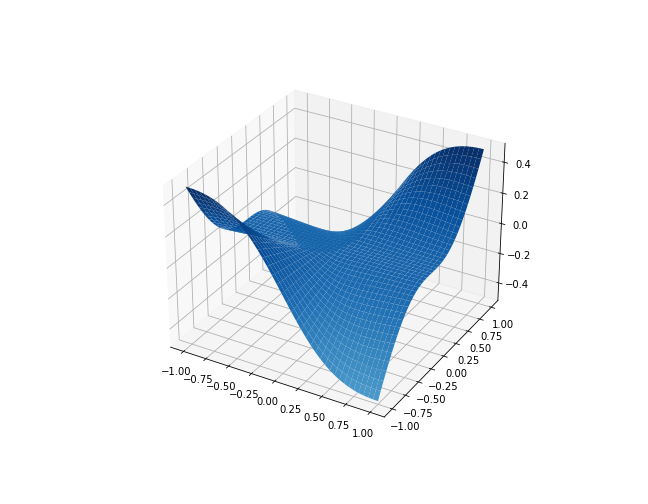
\includegraphics[width=\textwidth]{non_interchangeable_partial_derivatives}
    \caption{\( f(x,y) = xy^3/(x^2 + y^2) \)}\label{fig:non_interchangeable_partial_derivatives}
\end{figure}
\bigskip

\begin{remark}
    The existence of the partial derivatives does not guarantee differentiability. Let \( f(0,y) = 0 \) and
    \[
        f(x,y) = \frac{y^3}{x^2 + y^2}
    \]
    elsewhere. Then
    \[
        \partial_x f(x,y) = \frac{-2xy^3}{{(x^2 + y^2)}^2} \spacedtext{and}
        \partial_y f(x,y) = \frac{3x^2y^2 + y^4}{{(x^2 + y^2)}^2}
    \]
    % \begin{calculation}
    %     \frac{\partial f}{\partial y}(x,y) = \frac{3x^2y^2 + y^4}{{(x^2 + y^2)}^2}
    %     \frac{\partial f}{\partial y}(x,y) = \frac{3y^2(x^2 + y^2) - 2y^3y}{{(x^2 + y^2)}^2}
    %     = \frac{3x^2y^2 + y^4}{{(x^2 + y^2)}^2}
    % \end{calculation}
    Thus \( \partial_x f (x, 0) = 0 \) and \( \partial_y f (0,y) = 1 \), hence
    \( \gradient f(0,0) = (0, 1) \). But for \( t > 0 \)
    \[
        \frac{|f(t,t) - f(0,0) - \gradient f(0,0) (t,t)|}{\|(t,t)\|}
        = \frac{|\frac{1}{2t} - t|}{\sqrt{2}t} = \frac{1}{2\sqrt{2}}
    \]
\end{remark}
\bigskip


\begin{figure}[H]
    \centering
    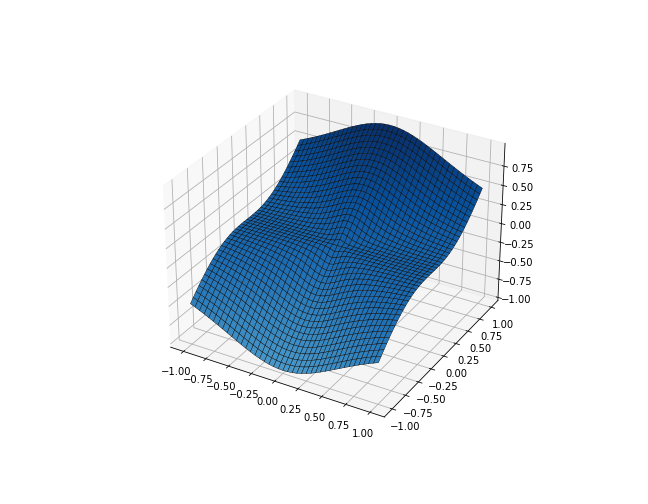
\includegraphics[width=\textwidth]{partial_derivatives_but_not_differentiable}
    \caption{\( f(x,y) = y^3/(x^2 + y^2) \)}\label{fig:partial_derivatives_but_not_differentiable}
\end{figure}
\bigskip


\begin{lemma}
    Let \( f: \Rn \to \R \) and \( g: \Rm \to \Rn \).
    \begin{enumerate}
        \item The partial derivatives of the composed mapping are given by the following equation
              \[
                  \partial_j (f \circ g) (x) = \sum_{k=1}^n \partial_k f(g(x))\,\partial_j g_k(x)
              \]
        \item The special case \( n = 1 \) yields
              \[
                  \partial_j (f \circ g) (x) = f'(g(x))\,\partial_j g_k(x)
              \]
    \end{enumerate}
\end{lemma}
\bigskip


\begin{examples}\hfill
    \begin{enumerate}
        \item Consider the norm \( r(x) = \|x\| = \sqrt{x_1^2 + x_2^2 \dots x_n^2} \). Then the chain rule yields
              \[
                  \partial_j r(x) = \frac{2 x_j}{2 \sqrt{x_1^2 + x_2^2 \dots x_n^2}} = \frac{x_j}{\|x\|}
              \]
              and \( r \) is differentiable on \( \Rn {\setminus} \{ 0 \} \).
        \item For \( f \) differentiable follows
              \[
                  \partial_j (f \circ r)(x) = \frac{f'(r(x))}{\|x\|} x_j
              \]
    \end{enumerate}
\end{examples}
\bigskip


\begin{lemma}[Directional Derivative]\label{lemma:directional_derivative}
    Let \( \Omega \subseteq \Rn \) be open and \( f \in C^1(\Omega) \). Then
    \[
        \partial_v f(x) = \gradient{f(x)}^T v
    \]
    for any \( v \in \Rn \).
\end{lemma}

\begin{proof}
    Let \( \varphi(t) = f(x + tv) \). Then \( \varphi \in C^1[-\eps, \eps ] \) for some \( \eps > 0 \)
    and the chain rule yields
    \[
        \varphi'(t) = {\gradient f(x + tv)}^T v
    \]
    Hence
    \[
        \varphi'(0) = \lim_{t \to 0} \frac{\varphi(x + tv) - \varphi(0)}{t} =
        \lim_{t \to 0} \frac{f(x + tv) - f(x)}{t} = {\gradient f(x)}^T v
    \]
\end{proof}
\bigskip


\begin{remarks}\hfill
    \begin{enumerate}
        \item A similar proposition holds under the weaker assumption that \( v \) is a only feasable direction
              for \( f \) in \( x \)
        \item For \( v = \gradient{f(x)}/\| \gradient{f(x)}\| \) it follows that
              \[
                  \partial_v f (x) = \|\gradient{f(x)}\| > 0
              \]
              and for any other \( v \in \Rn \) with \( \|v\| = 1 \) the Cauchy Schwarz inequality yields
              \[
                  \left|\partial_v f(x)\right| = |\gradient{f(x)}^T v|
                  \le \|\gradient{f(x)}\| \|v\| =\|\gradient{f(x)}\|
              \]
              Hence \( \gradient{f(x)} \) is the direction of the greatest ascent and respectively
              \( -\gradient{f(x)} \) is the direction of the greatest descent.
    \end{enumerate}
\end{remarks}
\bigskip


\begin{theorem}[First Order Necessary Condition]\label{thm:fonc}
    Let \( \Omega \subseteq \Rn \) be open and \( f \in C^1(\Omega) \). If \( x^* \in \Omega \) is a local minimzer then
    \( \gradient f(x^*) = 0 \).
\end{theorem}

\begin{proof}
    Let \( v \in \Rn \) and \( \delta > 0 \) so that \( x^* + tv \in \Omega \) for all \( t \in (-\delta, \delta) \).
    Then \( 0 \) is local minimizer for \( \varphi(t) = f(x^* + tv) \) and
    \[
        \varphi'(0) = {\gradient f(x^*)}^T v = 0
    \]
    Now let \( v = \gradient f(x^*) \).
\end{proof}
\bigskip


\begin{theorem}[Banach Fixed-Point Theorem]\label{thm:banach_fix_point}
    Let \( X \) be a Banach space and \( f \in C(X,X) \) a contraction
    \[
        \|f(x) - f(y)\| \le q \|x - y\| \text{ for all } x, y \in X
    \]
    for some \( 0 < q < 1 \). Then there exists a unique fix point \( x^* \in X \) with
    \[
        f(x^*) = x^*
    \]
    Furthermore for any \( x_0 \in X \) the sequence defined by
    \[
        x_{n+1} = f(x_n)
    \]
    converges aganist \( x^* \).
\end{theorem}

\begin{proof}
    Since \( \| x_{n+1} - x_n\| =\| f(x_n) - f(x_{n-1})\| \le q\| x_n - x_{n-1}\| \) it follows, that
    \[
        \| x_{n+1} - x_n\| \le q^n  \|x_1 - x_0\|
    \]
    Furthermore
    \[
        \| x_n - x_m\| \le \sum_{k=m}^n q^k \|x_1 - x_0\| = \frac{q^m - q^{n+1}}{1 - q} \|x_1 - x_0\|
    \]
    and \( (x_n) \) is a Cauchy sequence. For its limit \( x^* \) it follows
    \[
        x^* = \lim_{n\to\infty} x_{n+1} = \lim_{n\to\infty} f(x_n) = f(x^*)
    \]
    For any other \( y^* \in X \) with \( f(y^*) = y^* \) it follows, that
    \[
        \|x^* - y^*\| = \|f(x^*) - f(y^*)\| \le q \|x^* - y^*\|
    \]
    and therefore \( x^* = y^*\).

\end{proof}
\bigskip

